\section{Synthetic Datasets for AL}

AL approaches can be categorized into two types, uncertainty \cite{wang2014new, gal2017deep} - and geometric-approaches \cite{sener2017active, hacohen2022active, ashdeep}. Both types have principled shortcomings in terms of the utilized information that makes them unsuitable for certain data distributions. To test for these specific shortcomings, we created two synthetic datasets, namely "Honeypot" and "Diverging Sine", that are hard to solve for methods focused on the classifier's decision boundary or data clustering respectively. 
To avoid algorithms memorizing these datasets they are generated from scratch for each experiment, depending on $s_\D$. \\
\begin{figure}[H]
	\centering
	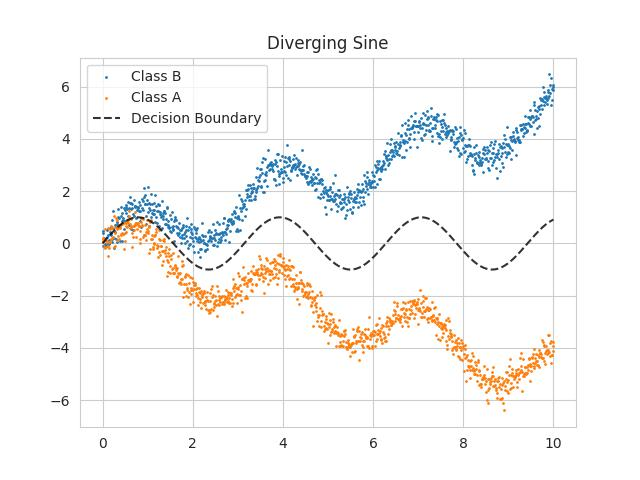
\includegraphics[width=0.4\linewidth]{img/diverging_sin.jpg}
	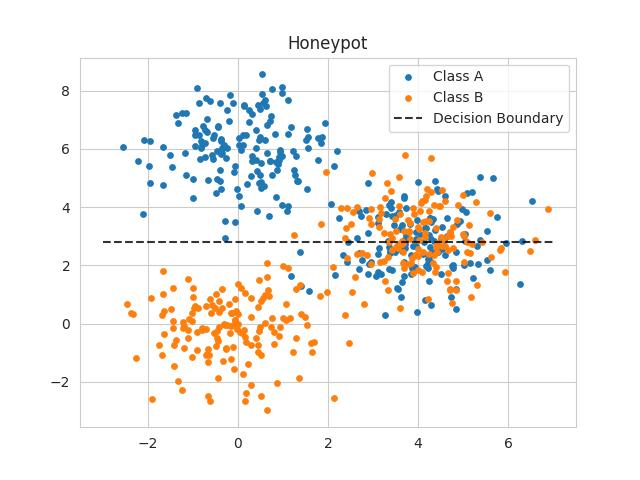
\includegraphics[width=0.4\linewidth]{img/honeypot.jpg}
	\caption{Synthetic "Honeypot" and "Diverging Sine" datasets. The optimal decision boundary is not part of the dataset and serves only as a visual guide.}
	\label{fig:synthDataAppendix}
\end{figure}

\begin{wraptable}{R}{0.65\textwidth}
	\vspace{-0.7cm}
	\caption{Overview of available batch sizes for our synthetic datasets}
	\vspace{0.1cm}
	\label{tab:batch_sizes_syn}
	\begin{tabular}{l|c|c|c|c|c|c|c|c}
		& B & 1 & 5 & 20 & 50 & 100 & 500 & 1000 \\
		\hline
		Honeypot    & 60 & o & o &&&&& \\
		Diverging Sine& 60 & o & o &&&&& \\
	\end{tabular}
	\vspace{-0.35cm}
\end{wraptable}
Honeypot creates to two easy to distinguish clusters with 150 samples each and one overlapping "honeypot" that represents a noisy region of the dataset with potentially miss-labeled, miss-measured or generally adverse samples.
This honeypot contains 150 samples of each class, creating a balance of 50\% beneficial samples and 50\% adverse samples in the dataset.
The honeypot is located on the likely decision boundary of a classifier that is trained on the beneficial samples to maximize its negative impact on purely uncertainty based acquisition functions.
Diverging Sine samples the datapoints for each class from two diverging sinusoidal functions that are originating from the same y-intercept.
This creates a challenging region one the left hand side, where a lot of datapoints need to be sampled and an easy region on the right hand side, where very few datapoints are enough. 
The repeating nature of a sin function encourages diversity based acquisition functions to equally sample the entire length, drastically oversampling the right hand side of the dataset.
Each class has 500 datapoints. The available batch sizes for our proposed datasets are shown in Table \ref{tab:batch_sizes_syn}.\\





Results for the Honeypot dataset reveal expected shortcomings of uncertainty sampling algorithms like margin, entropy and least confident sampling as well as BALD.
In addition, BADGE is underperforming for this dataset compared to real-world data. 
Results for Diverging Sine also confirm expected behavior, as clustering algorithms (Coreset, TypiClust) fall behind uncertainty algorithms (Entropy-, Margin-Sampling), with the exception of BADGE. \\
We provide a very small ablation study on the importance of the embeddings by testing a version of Coreset and TypiClust on this dataset that does not use the embeddings produced by the classification model, but rather clusters the data directly.
"Coreset Raw" and "TypiClust Raw" both perform worse than their embedding-based counterpart.

\begin{figure}
	\centering
	\caption{Results for all acquisition functions on both synthetic datasets.}
	\label{fig:main_body_result}
	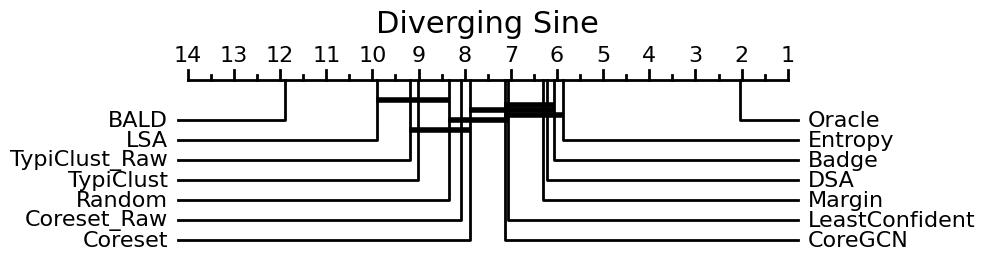
\includegraphics[width=0.49\linewidth]{img/micro_diverging_sin.jpg}
	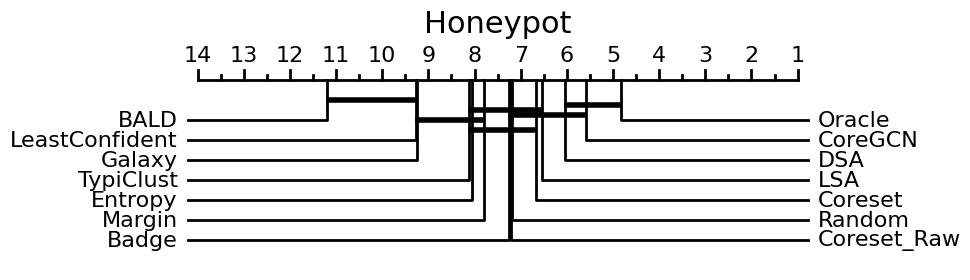
\includegraphics[width=0.49\linewidth]{img/micro_honeypot.jpg}
\end{figure}
